\documentclass[a4paper]{oblivoir}
\usepackage{amsmath,amssymb,kotex,kswrapfig,mdframed,paralist}
\usepackage{fapapersize}
\usefapapersize{210mm,297mm,20mm,*,20mm,*}

\usepackage{tabto,pifont}
\TabPositions{0.2\textwidth,0.4\textwidth,0.6\textwidth,0.8\textwidth}
\newcommand\tabb[5]{\par\noindent
\ding{172}\:{\ensuremath{#1}}
\tab\ding{173}\:\:{\ensuremath{#2}}
\tab\ding{174}\:\:{\ensuremath{#3}}
\tab\ding{175}\:\:{\ensuremath{#4}}
\tab\ding{176}\:\:{\ensuremath{#5}}}

\usepackage{graphicx}

%\pagestyle{empty}

%%% Counters
\newcounter{num}

%%% Commands
\newcommand\prob[1]
{\vs\bigskip\bigskip\par\noindent\stepcounter{num} \textbf{문제 \thenum) #1}\par\noindent}

\newcommand\pb[1]{\ensuremath{\fbox{\phantom{#1}}}}

\newcommand\ba{\ensuremath{\:|\:}}

\newcommand\vs[1]{\vspace{40pt}}

\newcommand\an[1]{\bigskip\par\noindent\textbf{문제 #1)}\par\noindent}

%%% Meta Commands
\let\oldsection\section
\renewcommand\section{\clearpage\oldsection}

\let\emph\textsf

\begin{document}
\begin{center}
\LARGE준영, 미니테스트 21
\end{center}
\begin{flushright}
날짜 : 2017년 \(\pb3\)월 \(\pb{10}\)일 \(\pb{월}\)요일
,\qquad
제한시간 : \pb{17년}분
,\qquad
점수 : \pb{20} / \pb{20}
\end{flushright}

%
\prob{}
두 함수 \(f(x)=x^3-1\), \(g(x)=4x+1\)에 대하여\\
\(\displaystyle\int F(x)\,dx=f(x)g(x)\)를 만족시키는 함수 \(F(x)\)가 있다.
\(F(1)\)의 값을 구하시오.
\par\bigskip
\tabb{-5}05{10}{15}

%
\prob{}
함수 \(f(x)=4x\)에 대하여
\[F(x)=\int f(x)\,dx+\frac d{dx}\int f(x)\,dx\]
가 \(x=k\)에서 최솟값을 가질 때, 상수 \(k\)의 값은?
\tabb{-2}{-1}012

%
\prob{}
삼차함수 \(f(x)\)의 도함수가 \(f'(x)=12x^2-20x+8\)이고 \(f(x)\)의 극솟값이 \(4\)일 때, \(f(-1)\)의 값은?
\tabb{-20}{-22}{-24}{-26}{-28}

%
\prob{}
\begin{minipage}{0.6\textwidth}
삼차함수 \(f(x)\)의 도함수 \(y=f'(x)\)의 그래프가 그림과 같다.
\(f(x)\)의 극댓값이 \(4\), 극솟값이 \(-8\)일 때, \(f(1)\)의 값은?
\end{minipage}
\begin{minipage}{0.3\textwidth}
\centering
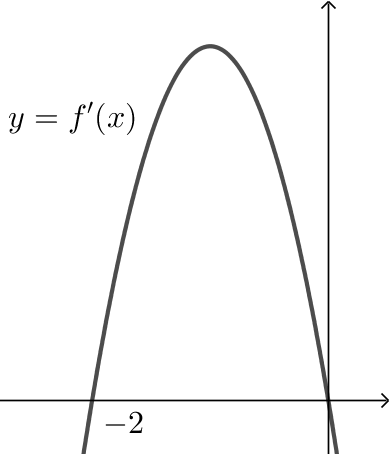
\includegraphics[width=0.5\textwidth]{y=-3x^2+6x}
\end{minipage}
\tabb{-8}{-7}{-6}{-5}{-4}

%
\prob{}
함수 \(\displaystyle f(x)=\int(x-2)^3\,dx+\int(x+2)^3\,dx\)에 대하여 \(f(2)=60\)일 때, \(f(0)\)의 값은?
\par\bigskip
\tabb1248{16}

%
\prob{}
다항함수 \(f(x)\)의 부정적분 중 하나가
\[F(x)=\frac14x^4-2x^3+3x^2+4x\]
일 때, 곡선 \(y=f(x)\) 위의 점 \((x,f(x))\)에서의 접선의 기울기의 최솟값은?
\tabb{-5}{-6}{-7}{-8}{-9}

%
\prob{}
미분가능한 함수 \(f(x)\)가 모든 실수 \(x\), \(y\)에 대하여
\[f(x+y)-f(x)=2axy+y+y^2\]
을 만족시키고 \(f(0)=2\), \(f(1)=4\)일 때, \(f(2)\)의 값은?
(단, \(a\)는 상수이다.)
\tabb56789

%
\prob{}
다항함수 \(f(x)\)가 \(\displaystyle f(x)=\frac d{dx}\int_a^x(2t^2-t+1)\,dt\)일 때, 곡선 \(y=f(x)\) 위의 점 \((-1,f(-1))\)에서의 접선의 \(y\)절편은?
(단, \(a\)는 상수이다.)
\tabb{-9}{-8}{-7}{-6}{-5}

%
\prob{}
등식 \(\displaystyle\int_1^{a+1}(4x+a)\,dx=a+6\)을 만족시키는 양수 \(a\)의 값은?
\par\bigskip
\tabb{\frac12}1{\frac32}2{\frac52}

%
\prob{}
\(\displaystyle\int_{-1}^2(x^2-4x)\,dx+\int_4^3x(4-x)\,dx-\int_3^2x(x-4)\,dx\)의 값은?
\par\bigskip
\tabb{-\frac{25}3}{-\frac{23}3}{-7}{-\frac{19}3}{-\frac{17}3}

%
\prob{}
\(\displaystyle\int_0^3|2x-x^2|\,dx\)의 값은?
\par\bigskip
\tabb{\frac43}2{\frac83}{\frac{10}3}4

%
\prob{}
연속함수 \(f(x)\)가 다음 조건을 만족시킬 때,\\
\(\displaystyle\int_0^2f(x)\,dx\)의 값은?
\begin{mdframed}
\begin{enumerate}[(가)]
\item
모든 실수 \(x\)에 대하여 \(f(-x)=f(x)\)가 성립한다.
\item
\(\displaystyle\int_{-4}^2f(x)\,dx=20,\quad\int_2^4f(x)\,dx=4\)
\end{enumerate}
\end{mdframed}
\par\bigskip
\tabb48{12}{16}{20}

%
\prob{}
\(\displaystyle\lim_{x\to-1}\frac4{x^2-1}\int_{-1}^x|t-1|\,dt\)의 값은?
\par\bigskip
\tabb{-10}{-8}{-6}{-4}{-2}

%
\prob{}
\(\displaystyle\lim_{n\to\infty}\frac4n\left[
\left(1+\frac2n\right)^3+\left(1+\frac4n\right)^3+\left(1+\frac6n\right)^3
+\cdots+\left(1+\frac{2n}n\right)^3\right]
\)의 값을 구하시오.
\par\bigskip
\tabb{10}{20}{30}{40}{50}

\end{document}